In this section, we first present the problem formulation of traffic matrix prediction under the lack of ground-truth input. 
Then, we give a brief introduction about the Long Short-Term Memory and Convolutional LSTM networks which are used in our approach. 
% We summarize the major notations in the table \ref{table:notations} for quick reference.
% \begin{table}[]
% \begin{tabular}{|c|l|}
% \hline
% Notations           & Description                                                                                                                                                              \\ \hline
% N                   & Set of node in the network. |N| = n.                                                                                                                                     \\ \hline
% X                   & The traffic matrix at timestep j                                                                                                                                         \\ \hline
% X$\sim$             & The predicted traffic matrix for timestep j                                                                                                                              \\ \hline
% x                   & Traffic volume of flow (s,d) at timesteps j. x \textbackslash{}in X                                                                                                      \\ \hline
% o                   & The ground-truth value of traffic volume of flow (s,d) at timestep j                                                                                                     \\ \hline
% x$\sim$             & The predicted traffic volume of flow (s,d) for timestep j.                                                                                                               \\ \hline
% x\textasciicircum{} & The predicted traffic volume of flow (s,d) for timestep j by backward network.                                                                                           \\ \hline
% m                   & \begin{tabular}[c]{@{}l@{}}The binary variable, m = 1 indicates that the traffic volume of flow\\  (s,d) at timestep j is ground-truth value and otherwise.\end{tabular} \\ \hline
% M                   & The measurement matrix at timestep j.                                                                                                                                    \\ \hline
% lf                  & The forward loss                                                                                                                                                         \\ \hline
% lb                  & The backward loss                                                                                                                                                        \\ \hline
% w                   & The weight of flow (s,d) is calculated at current timestep t.                                                                                                            \\ \hline
% \end{tabular}
% \caption{My caption}
% \label{my-label}
% \end{table}
\subsection{Problem Description}
\label{subsec:problem_description}
\begin{figure}
\centering
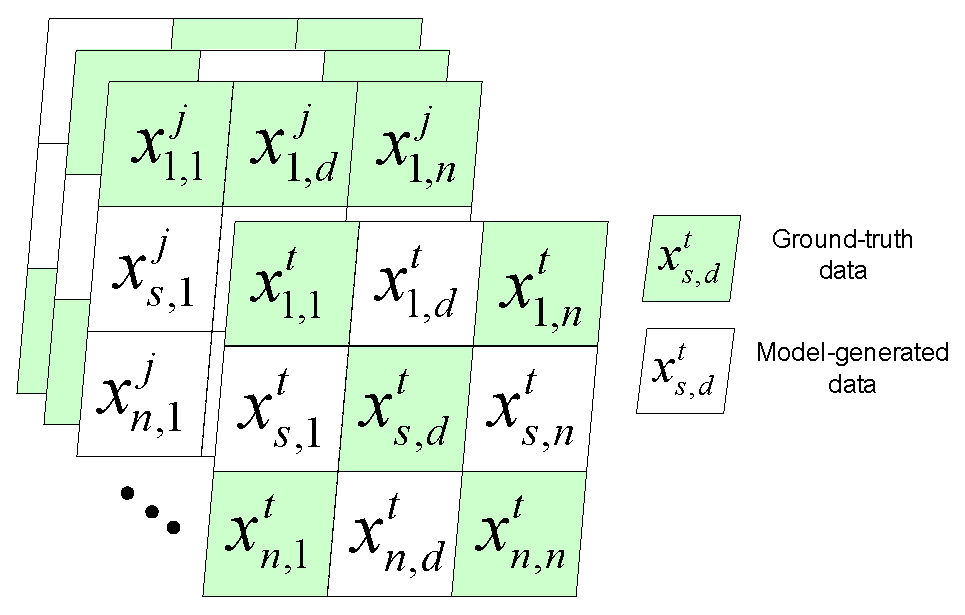
\includegraphics[width=0.6\columnwidth]{preliminaries_figs/traffic_matrices.eps}
		\caption{A sequence of $J$ previous traffic matrices including both ground-truth and imprecise data. \label{fig:traffic_matrices}}
\end{figure}
%\vskip -5ex
%\vspace{-10pt}
%In this section, we present the problem formulation of traffic prediction under the lack of precise input traffic data. 
We suppose that the traffic monitoring and predicting tasks are executed periodically in every \textit{timestep} and denote $t$ as the current timestep. Given a backbone network in which $\mathcal{N}$ is the set of nodes ($\left |  \mathcal{N} \right |=n$), let $X_j \in \mathbb{R}^{n \times n}$ be the traffic matrix at the timestep $j$. Each element $x_{s,d}^j \in X_j$  represents the traffic volume of a flow from a source $s$ to a destination $d$ in the network (flow ($s,d$), for short) at timestep $j$. Thus, the traffic matrix prediction problem is to estimate the traffic matrices of next $L$ timesteps (denoted by $\widetilde{X}_{t+1},...,\widetilde{X}_{t+L}$), given the previous $J$ measurements ($L,J \geq 1$):
\begin{equation}
\begin{aligned}
&\widetilde{X}_{t+1},...,\widetilde{X}_{t+L} \\
	&\quad = \argmax_{X_{t+1},...,X_{t+L}} p(X_{t+1},...,X_{t+L} | X_{t-J+1},...,X_{t})
\end{aligned}
\end{equation}
However, in this paper, we consider the case of backbone networks where we cannot obtain all the $J$ previous traffic matrices by directly monitoring all the flows. Although in recent years, advance network architectures such as Software-Defined Networking (SDN) \cite{mckeown2008openflow} and Network Function Virtualization (NFV) have enabled many alternative ways to measure the network flow information, collecting all the traffic statistics with low overhead (in terms of computational complexity, bandwidth, ...) still remains as a challenging task. Therefore, to reduce the monitoring overhead, we measure only a part of the traffic flows at each timestep and use the data generated by the prediction model to fill into the missed historical data.
%traffic matrix. 
Accordingly, the traffic matrix prediction problem under highly missing ground-truth data can be formulated as follows:

\textbf{Input}
\begin{equation}
\label{equation:tm_prediction_missing_data}
\begin{matrix}
x_{s,d}^{j}=\left\{\begin{matrix}
o_{s,d}^j & \text{if} \ m_{s,d}^j=1 \\
\widetilde{x}_{s,d}^j & \text{otherwise}
\end{matrix}\right. \\

\forall s, d \in N; j = t - J + 1,...,t 
\end{matrix}
\end{equation}

\textbf{Output}
\begin{equation}
\begin{aligned}
\widetilde{X}_{t+1}&,...,\widetilde{X}_{t+L} \\
	& = \argmax_{X_{t+1},...,X_{t+L}} p(X_{t+1},...,X_{t+L} |  X_{t-J+1},...,X_{t})
\end{aligned}
%\end{matrix}
\end{equation} 
where $o_{s,d}^j$ and $\widetilde{x}_{s,d}^j$ denote the observed and predicted value of flow ($s,d$) at timestep $j$, respectively. The binary variable $m_{s,d}^j$ depends on the monitoring policy, where $m_{s,d}^j = 1$ indicates that flow ($s,d$) is monitored at timestep $j$; otherwise, the value of traffic volume is filled up by the prediction result. Fig.\ref{fig:traffic_matrices} shows the sequence of $J$ previous traffic matrices which is used as the input for predicting the future traffic. The green elements are the ground-truth data obtained by monitoring the flows directly, and the white elements represent the predicted values.  
\subsection{LSTM and Convolutional LSTM network for spatiotemporal sequence modeling}
\label{subsection:lstm_ConvLSTM}
\begin{figure}		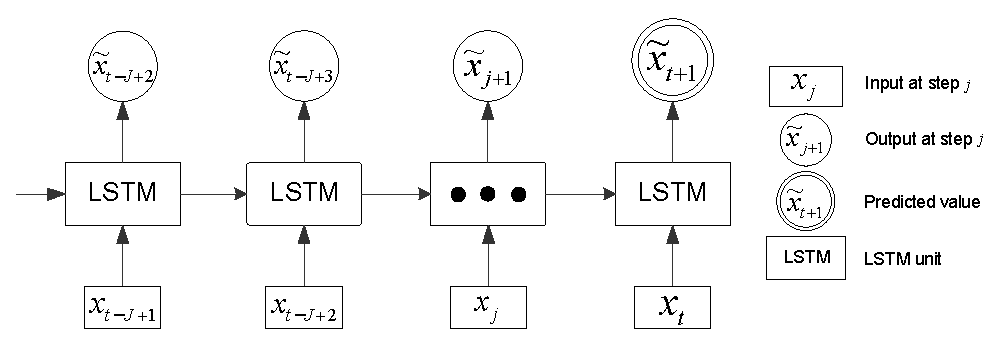
\includegraphics[width=0.8\columnwidth]{preliminaries_figs/LSTM_model.eps}
		\caption{The unfolded model of the LSTM network. \label{fig:LSTM_model}}
        %\vspace{-5pt}
\end{figure}
% \begin{figure}
% \centering
% 		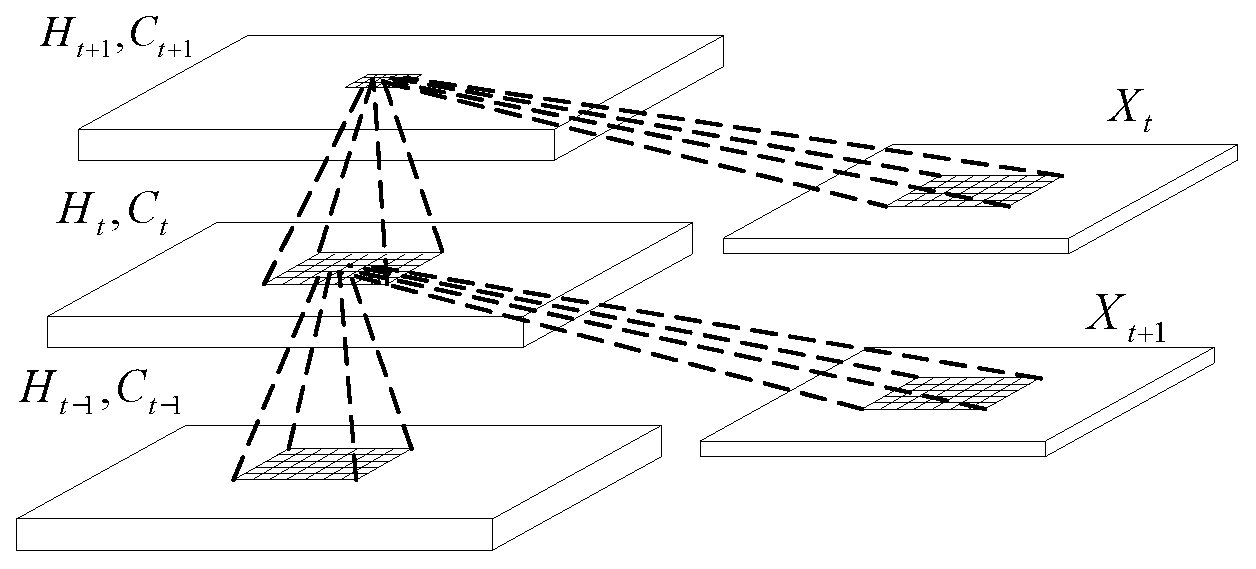
\includegraphics[width=0.65\columnwidth]{preliminaries_figs/ConvLSTM_model.eps}
% 		\caption{The inner structure of ConvLSTM network \cite{xingjian2015convolutional}. 
%         \label{fig:ConvLSTM_model}}
%         \vspace{-5pt}
% \end{figure}
Long Short-Term Memory network is a special Recurrent Neural Network which replaces the standard RNN units by the LSTM units. 
LSTM network has been proved to be stable and powerful for modeling long-range dependencies in various problem domains, thus it is well-suited for processing and making predictions based on time series or sequence data.
Indeed, LSTM has been applied in many real-life sequence modeling problems. 
The unfolded model of LSTM network (Fig.\ref{fig:LSTM_model}) shows that the input is processed step-by-step and the outputs of previous steps are used as the input for the next step. This architecture along with the advantages of the memory cell in LSTM units make LSTM network especially suitable for solving the series based predictions.

However, in many problems such as precipitation nowcasting \cite{xingjian2015convolutional} or images/videos based action prediction where the sequence data has a strong spatial relation, LSTM reveals many limitations. Therefore, to deal with more general spatiotemporal sequence forecasting problems, authors in \cite{xingjian2015convolutional} have proposed an extension of LSTM called ConvLSTM. The ConvLSTM layer has convolutional structures in both the input-to-state and state-to-state transitions which can exploit both temporal and spatial features of the input sequence. To obtain the spatiotemporal feature, the ConvLSTM network takes a 3D tensor $X_t$ as input in the processing step $t$, for example, $X_t$ can be a $32 \times 32 \times 3$ image whose the last dimension represents the color of the image (RGB). The key equations of the ConvLSTM are shown in (\ref{equation:convlstm}), where $i_t, f_t, o_t$ are the input, forget, output gates, respectively; $C_t, H_t$ are the cell and the final state of the LSTM unit, respectively; `$*$' denotes the convolution operator and `$\circ$' denotes the Hadamard product \cite{xingjian2015convolutional}:
\begin{equation}
\label{equation:convlstm}
\begin{aligned}
i_t &= \sigma(W_{xi}*X_t + W_{hi}*H_{t-1} + W_{ci}\circ C_{t-1} + b_i) \\
f_t &= \sigma(W_{xf}*X_t + W_{hf}*H_{t-1} + W_{cf}\circ C_{t-1} + b_f) \\
C_t &= f_t\circ C_{t-1} + i_t\circ \tanh(W_{xc}*X_t + W_{hc}*H_{t-1} + b_c) \\
o_t &= \sigma(W_{xo}*X_t + W_{ho}*H_{t-1} + W_{co}\circ C_{t} + b_o) \\
H_t &= o_t \circ \tanh(C_t)
\end{aligned}
\end{equation}
The main difference between the LSTM unit and ConvLSTM unit is the convolution operation (i.e., `$*$'). While the LSTM network only takes a 1D array as the input at each processing step, the ConvLSTM takes a 3D tensor as the input and uses multiple filters to extract the spatial information. The filter size (also called as kernel size) is $k \times k \times d$, where $k$ is an integer number (normally, $k=3,5,7,etc.$) and $d$ equals to the last dimension of the input. These filters are shifted across the 3D input, and hence, can extract the spatial features of the data.
